\documentclass[]{article}
\usepackage{lmodern}
\usepackage{amssymb,amsmath}
\usepackage{ifxetex,ifluatex}
\usepackage{listings}
\usepackage{fixltx2e} % provides \textsubscript
\ifnum 0\ifxetex 1\fi\ifluatex 1\fi=0 % if pdftex
  \usepackage[T1]{fontenc}
  \usepackage[utf8]{inputenc}
\else % if luatex or xelatex
  \ifxetex
    \usepackage{mathspec}
  \else
    \usepackage{fontspec}
  \fi
  \defaultfontfeatures{Ligatures=TeX,Scale=MatchLowercase}
  \newcommand{\euro}{€}
\fi
% use upquote if available, for straight quotes in verbatim environments
\IfFileExists{upquote.sty}{\usepackage{upquote}}{}
% use microtype if available
\IfFileExists{microtype.sty}{%
\usepackage{microtype}
\UseMicrotypeSet[protrusion]{basicmath} % disable protrusion for tt fonts
}{}
\usepackage[margin=1in]{geometry}
\usepackage{hyperref}
\PassOptionsToPackage{usenames,dvipsnames}{color} % color is loaded by hyperref
\hypersetup{unicode=true,
            pdftitle={Untitled},
            pdfauthor={Andre Guimaraes Duarte},
            pdfborder={0 0 0},
            breaklinks=true}
\urlstyle{same}  % don't use monospace font for urls
\usepackage{color}
\usepackage{fancyvrb}
\newcommand{\VerbBar}{|}
\newcommand{\VERB}{\Verb[commandchars=\\\{\}]}
\DefineVerbatimEnvironment{Highlighting}{Verbatim}{commandchars=\\\{\}}
% Add ',fontsize=\small' for more characters per line
\usepackage{framed}
\definecolor{shadecolor}{RGB}{248,248,248}
\newenvironment{Shaded}{\begin{snugshade}}{\end{snugshade}}
\newcommand{\KeywordTok}[1]{\textcolor[rgb]{0.13,0.29,0.53}{\textbf{{#1}}}}
\newcommand{\DataTypeTok}[1]{\textcolor[rgb]{0.13,0.29,0.53}{{#1}}}
\newcommand{\DecValTok}[1]{\textcolor[rgb]{0.00,0.00,0.81}{{#1}}}
\newcommand{\BaseNTok}[1]{\textcolor[rgb]{0.00,0.00,0.81}{{#1}}}
\newcommand{\FloatTok}[1]{\textcolor[rgb]{0.00,0.00,0.81}{{#1}}}
\newcommand{\ConstantTok}[1]{\textcolor[rgb]{0.00,0.00,0.00}{{#1}}}
\newcommand{\CharTok}[1]{\textcolor[rgb]{0.31,0.60,0.02}{{#1}}}
\newcommand{\SpecialCharTok}[1]{\textcolor[rgb]{0.00,0.00,0.00}{{#1}}}
\newcommand{\StringTok}[1]{\textcolor[rgb]{0.31,0.60,0.02}{{#1}}}
\newcommand{\VerbatimStringTok}[1]{\textcolor[rgb]{0.31,0.60,0.02}{{#1}}}
\newcommand{\SpecialStringTok}[1]{\textcolor[rgb]{0.31,0.60,0.02}{{#1}}}
\newcommand{\ImportTok}[1]{{#1}}
\newcommand{\CommentTok}[1]{\textcolor[rgb]{0.56,0.35,0.01}{\textit{{#1}}}}
\newcommand{\DocumentationTok}[1]{\textcolor[rgb]{0.56,0.35,0.01}{\textbf{\textit{{#1}}}}}
\newcommand{\AnnotationTok}[1]{\textcolor[rgb]{0.56,0.35,0.01}{\textbf{\textit{{#1}}}}}
\newcommand{\CommentVarTok}[1]{\textcolor[rgb]{0.56,0.35,0.01}{\textbf{\textit{{#1}}}}}
\newcommand{\OtherTok}[1]{\textcolor[rgb]{0.56,0.35,0.01}{{#1}}}
\newcommand{\FunctionTok}[1]{\textcolor[rgb]{0.00,0.00,0.00}{{#1}}}
\newcommand{\VariableTok}[1]{\textcolor[rgb]{0.00,0.00,0.00}{{#1}}}
\newcommand{\ControlFlowTok}[1]{\textcolor[rgb]{0.13,0.29,0.53}{\textbf{{#1}}}}
\newcommand{\OperatorTok}[1]{\textcolor[rgb]{0.81,0.36,0.00}{\textbf{{#1}}}}
\newcommand{\BuiltInTok}[1]{{#1}}
\newcommand{\ExtensionTok}[1]{{#1}}
\newcommand{\PreprocessorTok}[1]{\textcolor[rgb]{0.56,0.35,0.01}{\textit{{#1}}}}
\newcommand{\AttributeTok}[1]{\textcolor[rgb]{0.77,0.63,0.00}{{#1}}}
\newcommand{\RegionMarkerTok}[1]{{#1}}
\newcommand{\InformationTok}[1]{\textcolor[rgb]{0.56,0.35,0.01}{\textbf{\textit{{#1}}}}}
\newcommand{\WarningTok}[1]{\textcolor[rgb]{0.56,0.35,0.01}{\textbf{\textit{{#1}}}}}
\newcommand{\AlertTok}[1]{\textcolor[rgb]{0.94,0.16,0.16}{{#1}}}
\newcommand{\ErrorTok}[1]{\textcolor[rgb]{0.64,0.00,0.00}{\textbf{{#1}}}}
\newcommand{\NormalTok}[1]{{#1}}
\usepackage{graphicx,grffile}
\makeatletter
\def\maxwidth{\ifdim\Gin@nat@width>\linewidth\linewidth\else\Gin@nat@width\fi}
\def\maxheight{\ifdim\Gin@nat@height>\textheight\textheight\else\Gin@nat@height\fi}
\makeatother
% Scale images if necessary, so that they will not overflow the page
% margins by default, and it is still possible to overwrite the defaults
% using explicit options in \includegraphics[width, height, ...]{}
\setkeys{Gin}{width=\maxwidth,height=\maxheight,keepaspectratio}
\setlength{\parindent}{0pt}
\setlength{\parskip}{6pt plus 2pt minus 1pt}
\setlength{\emergencystretch}{3em}  % prevent overfull lines
\providecommand{\tightlist}{%
  \setlength{\itemsep}{0pt}\setlength{\parskip}{0pt}}
\setcounter{secnumdepth}{0}

%%% Use protect on footnotes to avoid problems with footnotes in titles
\let\rmarkdownfootnote\footnote%
\def\footnote{\protect\rmarkdownfootnote}

%%% Change title format to be more compact
\usepackage{titling}

% Create subtitle command for use in maketitle
\newcommand{\subtitle}[1]{
  \posttitle{
    \begin{center}\large#1\end{center}
    }
}

\setlength{\droptitle}{-2em}
  \title{MSAN 502 - Homework 2}
  \pretitle{\vspace{\droptitle}\centering\huge}
  \posttitle{\par}
  \author{Andre Guimaraes Duarte}
  \preauthor{\centering\large\emph}
  \postauthor{\par}
  \predate{\centering\large\emph}
  \postdate{\par}
  \date{July 27, 2016}



% Redefines (sub)paragraphs to behave more like sections
\ifx\paragraph\undefined\else
\let\oldparagraph\paragraph
\renewcommand{\paragraph}[1]{\oldparagraph{#1}\mbox{}}
\fi
\ifx\subparagraph\undefined\else
\let\oldsubparagraph\subparagraph
\renewcommand{\subparagraph}[1]{\oldsubparagraph{#1}\mbox{}}
\fi

\begin{document}
\maketitle

\section*{1}
My previous version of the \textbf{eliminate} algorithm was built around a big \texttt{for} loop (\textit{for every row in matrix A, perform elimination on next rows...}). While this works fine for \"perfect\" scenarios, it was not versatile enough to bypass temporary failures. In order to account for them, and therefore allow permutations, I had to modify my code into a big \texttt{while} loop (\textit{while we haven't reached the bottom of matrix A, perform elimination. If we can't, try permuation}). My \texttt{Eliminate.py} file is commented well enough (in my humble opinion) for someone to understand what every line is doing.

Some big changes comparing to the previous version is that my algorithm now accepts non-square matrices (although it is still not entirely useful for this week's assignment). $n \times n$ cases are handled fairly well in my tests. I have a few checks in place as well, to make sure that everything is set up correctly in order for my algorithm to work without hiccups (A and b must be instances of \texttt{np.array}, their dimensions must match, etc).

My code solves $Ax = b$ when there is a unique solution, even if permutations of rows are needed. Print statements (original matrix, reduced matrix, solution vector, etc) have been commented out in order to run the complexity problem below, but can be de-commented as needed.

My algorithm runs into a permanent failure if the \textbf{solvability check} fails. This means that, at one point in the algorithm, we reached a row where we have $0$ on the left side of the equation and $c \neq 0$ on the right side, which is an impossibility. By calculating the number of pivots and comparing to the number of columns, I also have the number of special solutions.

If there are no special solutions, then it means there is only one solution. In the other case, there are infinitely many solutions. Again, print statements may have been commented out in order to run the complexity problem. In both of these cases, my algorithm runs to the end. If there is only one solution, backwards substitution finds the unique solution. I haven't yet integrated the scenario of infinitely many solutions (finding the particular and special solutions).

\section*{2}
Time complexity of my implementation of this algorithm can be found in \texttt{complexity.py}. I run my algorithm ten times to solve $Ax = b$, where $A$ is a $n \times n$ matrix with random noise for $n = 2^k$, where $k \in [2; 12]$. I save the average run time for each $n$.

Then, I use \texttt{complexity\_plot.py} to plot $\log{time}$ as a function of $\log{n}$. The resulting plot is shown in figure \ref{complexity}.

\begin{figure}[h]
\centering
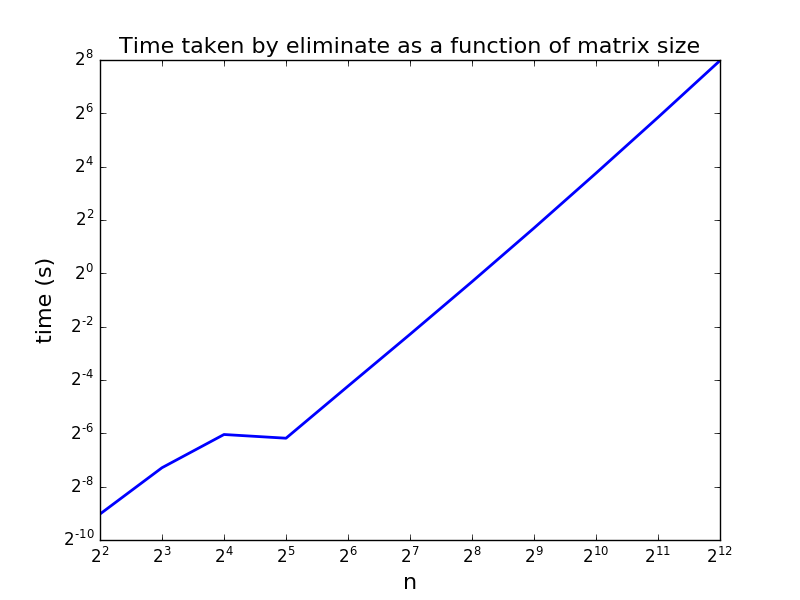
\includegraphics{complexity.png}
\caption{Time complexity of eliminate algorithm}
\label{complexity}
\end{figure}

We can see that there seems to be a linear correlation between $\log{time}$ and $\log{n}$. The slope of the most linear part (between $n = 128$ and $n = 4096$), the slope is $\frac{\Delta y}{\Delta x} = 2.05$. Since we have plotted a log-log curve of the time taken by the algorithm as a function of $n$, the slope is actually equal to the run time complexity. Therefore, empirically, the run time complexity of my implementation of the elimination algorithm is $O(n^2)$. This result is actually rather surprising, since we know that the complexity of the full \textit{eliminate} algorithm is $O(n^3)$. To the best of my knowledge, I am performing the algorithm in its entirety, so there are four possibilities:

\begin{itemize}
\item Either I didn't implement the elimination algorithm in its entirety (but I honestly don't think this is the case),
\item or some functions that I am using are very well optimized in python, which brings the time complexity down,
\item or there is a difference between computational complexity and run time complexity,
\item or I should run this test for even bigger $n$s in order to reach the full complexity of the algorithm.
\end{itemize}

Either way, I am happy with the way my implementation is working. Now I only need to implement a function that finds the particular and special solutions, in order for the program to fail only when there are no solutions (the solvability check fails)!

\end{document}
